\documentclass{ximera}

%\usepackage{todonotes}

\newcommand{\todo}{}

\usepackage{esint} % for \oiint
\ifxake%%https://math.meta.stackexchange.com/questions/9973/how-do-you-render-a-closed-surface-double-integral
\renewcommand{\oiint}{{\large\bigcirc}\kern-1.56em\iint}
\fi


\graphicspath{
  {./}
  {ximeraTutorial/}
  {basicPhilosophy/}
  {functionsOfSeveralVariables/}
  {normalVectors/}
  {lagrangeMultipliers/}
  {vectorFields/}
  {greensTheorem/}
  {shapeOfThingsToCome/}
  {dotProducts/}
  {partialDerivativesAndTheGradientVector/}
  {../productAndQuotientRules/exercises/}
  {../normalVectors/exercisesParametricPlots/}
  {../continuityOfFunctionsOfSeveralVariables/exercises/}
  {../partialDerivativesAndTheGradientVector/exercises/}
  {../directionalDerivativeAndChainRule/exercises/}
  {../commonCoordinates/exercisesCylindricalCoordinates/}
  {../commonCoordinates/exercisesSphericalCoordinates/}
  {../greensTheorem/exercisesCurlAndLineIntegrals/}
  {../greensTheorem/exercisesDivergenceAndLineIntegrals/}
  {../shapeOfThingsToCome/exercisesDivergenceTheorem/}
  {../greensTheorem/}
  {../shapeOfThingsToCome/}
  {../separableDifferentialEquations/exercises/}
}

\newcommand{\mooculus}{\textsf{\textbf{MOOC}\textnormal{\textsf{ULUS}}}}

\usepackage{tkz-euclide}\usepackage{tikz}
\usepackage{tikz-cd}
\usetikzlibrary{arrows}
\tikzset{>=stealth,commutative diagrams/.cd,
  arrow style=tikz,diagrams={>=stealth}} %% cool arrow head
\tikzset{shorten <>/.style={ shorten >=#1, shorten <=#1 } } %% allows shorter vectors

\usetikzlibrary{backgrounds} %% for boxes around graphs
\usetikzlibrary{shapes,positioning}  %% Clouds and stars
\usetikzlibrary{matrix} %% for matrix
\usepackage{pgfplots}
\usepgfplotslibrary{polar} %% for polar plots
\usepgfplotslibrary{fillbetween} %% to shade area between curves in TikZ
\usetkzobj{all}
\usepackage[makeroom]{cancel} %% for strike outs
%\usepackage{mathtools} %% for pretty underbrace % Breaks Ximera
%\usepackage{multicol}
\usepackage{pgffor} %% required for integral for loops



%% http://tex.stackexchange.com/questions/66490/drawing-a-tikz-arc-specifying-the-center
%% Draws beach ball
\tikzset{pics/carc/.style args={#1:#2:#3}{code={\draw[pic actions] (#1:#3) arc(#1:#2:#3);}}}



\usepackage{array}
\setlength{\extrarowheight}{+.1cm}
\newdimen\digitwidth
\settowidth\digitwidth{9}
\def\divrule#1#2{
\noalign{\moveright#1\digitwidth
\vbox{\hrule width#2\digitwidth}}}





\newcommand{\RR}{\mathbb R}
\newcommand{\R}{\mathbb R}
\newcommand{\N}{\mathbb N}
\newcommand{\Z}{\mathbb Z}

\newcommand{\sagemath}{\textsf{SageMath}}


%\renewcommand{\d}{\,d\!}
\renewcommand{\d}{\mathop{}\!d}
\newcommand{\dd}[2][]{\frac{\d #1}{\d #2}}
\newcommand{\pp}[2][]{\frac{\partial #1}{\partial #2}}
\renewcommand{\l}{\ell}
\newcommand{\ddx}{\frac{d}{\d x}}

\newcommand{\zeroOverZero}{\ensuremath{\boldsymbol{\tfrac{0}{0}}}}
\newcommand{\inftyOverInfty}{\ensuremath{\boldsymbol{\tfrac{\infty}{\infty}}}}
\newcommand{\zeroOverInfty}{\ensuremath{\boldsymbol{\tfrac{0}{\infty}}}}
\newcommand{\zeroTimesInfty}{\ensuremath{\small\boldsymbol{0\cdot \infty}}}
\newcommand{\inftyMinusInfty}{\ensuremath{\small\boldsymbol{\infty - \infty}}}
\newcommand{\oneToInfty}{\ensuremath{\boldsymbol{1^\infty}}}
\newcommand{\zeroToZero}{\ensuremath{\boldsymbol{0^0}}}
\newcommand{\inftyToZero}{\ensuremath{\boldsymbol{\infty^0}}}



\newcommand{\numOverZero}{\ensuremath{\boldsymbol{\tfrac{\#}{0}}}}
\newcommand{\dfn}{\textbf}
%\newcommand{\unit}{\,\mathrm}
\newcommand{\unit}{\mathop{}\!\mathrm}
\newcommand{\eval}[1]{\bigg[ #1 \bigg]}
\newcommand{\seq}[1]{\left( #1 \right)}
\renewcommand{\epsilon}{\varepsilon}
\renewcommand{\phi}{\varphi}


\renewcommand{\iff}{\Leftrightarrow}

\DeclareMathOperator{\arccot}{arccot}
\DeclareMathOperator{\arcsec}{arcsec}
\DeclareMathOperator{\arccsc}{arccsc}
\DeclareMathOperator{\si}{Si}
\DeclareMathOperator{\scal}{scal}
\DeclareMathOperator{\sign}{sign}


%% \newcommand{\tightoverset}[2]{% for arrow vec
%%   \mathop{#2}\limits^{\vbox to -.5ex{\kern-0.75ex\hbox{$#1$}\vss}}}
\newcommand{\arrowvec}[1]{{\overset{\rightharpoonup}{#1}}}
%\renewcommand{\vec}[1]{\arrowvec{\mathbf{#1}}}
\renewcommand{\vec}[1]{{\overset{\boldsymbol{\rightharpoonup}}{\mathbf{#1}}}}
\DeclareMathOperator{\proj}{\mathbf{proj}}
\newcommand{\veci}{{\boldsymbol{\hat{\imath}}}}
\newcommand{\vecj}{{\boldsymbol{\hat{\jmath}}}}
\newcommand{\veck}{{\boldsymbol{\hat{k}}}}
\newcommand{\vecl}{\vec{\boldsymbol{\l}}}
\newcommand{\uvec}[1]{\mathbf{\hat{#1}}}
\newcommand{\utan}{\mathbf{\hat{t}}}
\newcommand{\unormal}{\mathbf{\hat{n}}}
\newcommand{\ubinormal}{\mathbf{\hat{b}}}

\newcommand{\dotp}{\bullet}
\newcommand{\cross}{\boldsymbol\times}
\newcommand{\grad}{\boldsymbol\nabla}
\newcommand{\divergence}{\grad\dotp}
\newcommand{\curl}{\grad\cross}
%\DeclareMathOperator{\divergence}{divergence}
%\DeclareMathOperator{\curl}[1]{\grad\cross #1}
\newcommand{\lto}{\mathop{\longrightarrow\,}\limits}

\renewcommand{\bar}{\overline}

\colorlet{textColor}{black}
\colorlet{background}{white}
\colorlet{penColor}{blue!50!black} % Color of a curve in a plot
\colorlet{penColor2}{red!50!black}% Color of a curve in a plot
\colorlet{penColor3}{red!50!blue} % Color of a curve in a plot
\colorlet{penColor4}{green!50!black} % Color of a curve in a plot
\colorlet{penColor5}{orange!80!black} % Color of a curve in a plot
\colorlet{penColor6}{yellow!70!black} % Color of a curve in a plot
\colorlet{fill1}{penColor!20} % Color of fill in a plot
\colorlet{fill2}{penColor2!20} % Color of fill in a plot
\colorlet{fillp}{fill1} % Color of positive area
\colorlet{filln}{penColor2!20} % Color of negative area
\colorlet{fill3}{penColor3!20} % Fill
\colorlet{fill4}{penColor4!20} % Fill
\colorlet{fill5}{penColor5!20} % Fill
\colorlet{gridColor}{gray!50} % Color of grid in a plot

\newcommand{\surfaceColor}{violet}
\newcommand{\surfaceColorTwo}{redyellow}
\newcommand{\sliceColor}{greenyellow}




\pgfmathdeclarefunction{gauss}{2}{% gives gaussian
  \pgfmathparse{1/(#2*sqrt(2*pi))*exp(-((x-#1)^2)/(2*#2^2))}%
}


%%%%%%%%%%%%%
%% Vectors
%%%%%%%%%%%%%

%% Simple horiz vectors
\renewcommand{\vector}[1]{\left\langle #1\right\rangle}


%% %% Complex Horiz Vectors with angle brackets
%% \makeatletter
%% \renewcommand{\vector}[2][ , ]{\left\langle%
%%   \def\nextitem{\def\nextitem{#1}}%
%%   \@for \el:=#2\do{\nextitem\el}\right\rangle%
%% }
%% \makeatother

%% %% Vertical Vectors
%% \def\vector#1{\begin{bmatrix}\vecListA#1,,\end{bmatrix}}
%% \def\vecListA#1,{\if,#1,\else #1\cr \expandafter \vecListA \fi}

%%%%%%%%%%%%%
%% End of vectors
%%%%%%%%%%%%%

%\newcommand{\fullwidth}{}
%\newcommand{\normalwidth}{}



%% makes a snazzy t-chart for evaluating functions
%\newenvironment{tchart}{\rowcolors{2}{}{background!90!textColor}\array}{\endarray}

%%This is to help with formatting on future title pages.
\newenvironment{sectionOutcomes}{}{}



%% Flowchart stuff
%\tikzstyle{startstop} = [rectangle, rounded corners, minimum width=3cm, minimum height=1cm,text centered, draw=black]
%\tikzstyle{question} = [rectangle, minimum width=3cm, minimum height=1cm, text centered, draw=black]
%\tikzstyle{decision} = [trapezium, trapezium left angle=70, trapezium right angle=110, minimum width=3cm, minimum height=1cm, text centered, draw=black]
%\tikzstyle{question} = [rectangle, rounded corners, minimum width=3cm, minimum height=1cm,text centered, draw=black]
%\tikzstyle{process} = [rectangle, minimum width=3cm, minimum height=1cm, text centered, draw=black]
%\tikzstyle{decision} = [trapezium, trapezium left angle=70, trapezium right angle=110, minimum width=3cm, minimum height=1cm, text centered, draw=black]


\outcome{Recognize optimization problem.}
\outcome{Translate a word problem into the problem of finding the extreme values of a function.}
\outcome{Solve basic word problems involving maxima or minima.}
\outcome{Interpret an optimization problem as the procedure used to make a system or design as effective or functional as possible.}
\outcome{Set up an optimization problem by identifying the objective function and appropriate constraints.}
\outcome{Solve optimization problems by finding the appropriate absolute extremum.}
\outcome{Identify the appropriate domain for functions which are models of real-world phenomena.}

\title[Dig-In:]{Applied optimization}

\begin{document}
\begin{abstract}
  Now we put our optimization skills to work.
\end{abstract}
\maketitle


In this section, we will present several worked examples of
optimization problems. Our method for solving these problems is
essentially the following:
\begin{description}
\item[Draw a picture.] If possible, draw a schematic picture with all the relevant information. 
\item[Determine your goal.] We need identify what needs to be
  optimized.
\item[Find constraints.] What limitations are set on our
  optimization?
\item[Solve for a single variable.] Now you should have a function to optimize.
\item[Use calculus to find the extreme values.] Be sure to check your answer!
\end{description}






\begin{example}
You are making cylindrical containers to contain a given volume.  Suppose
that the top and bottom are made of a material that is $N$ times as
expensive (cost per unit area) as the material used for the lateral side of
the cylinder.  Find (in terms of $N$) the ratio of height to base radius of
the cylinder that minimizes the cost of making the containers.
\begin{explanation}
  First we draw a picture:
\begin{image}
  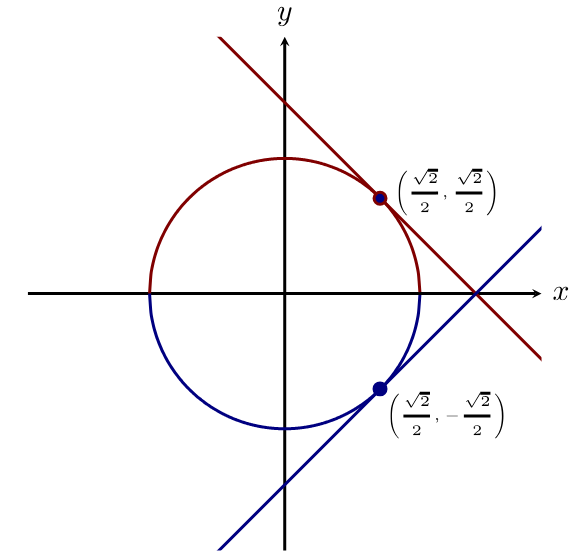
\includegraphics[scale=0.75]{2.png}
\end{image}
  Letting $c$ represent the cost of the lateral side, we can write an
  expression for the cost of materials:
  \[
  C = 2\pi c r h+2\pi r^{2}\answer[given]{Nc}.
  \]
  Since we know that $V=\pi r^2h$, we can use this relationship to
  eliminate $h$ (we could eliminate $r$, but it's a little easier if we
  eliminate $h$, which appears in only one place in the above formula
  for cost).  We find
\begin{align*}
  C(r)&=2c\pi r\frac{V}{\pi r^2}+2Nc\pi r^2\\
  &=\frac{2cV}{r}+2Nc\pi r^2.
\end{align*}
Since we have expressed the cost as a function of a single variable, the problem becomes a``calculus problem": Find the minimum of the function $C$ on the interval 
$(0,\infty)$.

 Although the function $C$ is continuous on its domain, its domain is an open, unbounded interval and the Extreme Value Theorem does not apply; there is no guarantee that the minimum even exists. But we don't give up! Our strategy will be to search for a critical point and check if the minimum is attained there. By solving the equation
\[
C'(r)=-2cV/r^2+4Nc\pi \answer[given]{r} =0
\]
we find that the point where $r=\sqrt[3]{V/(2N\pi)}$ is the only critical point of $C$.  Since $C''(r)=4cV/r^3+4Nc\pi$ is
positive when $r$ is positive, there is a local minimum at the
critical point, and hence a global minimum since there is only one
critical point.

Another way to reach this conclusion is to examine the sign of the derivative $C'(r)$ on the interval $(0,\infty)$:
\[
C'(r)=-2cV/r^2+4Nc\pi r=\frac{4Nc\pi (r^3-\frac{V}{2N\pi})}{r^2}. 
\]
From this factorization it is clear that $C'(r)<0$ on $(0,\sqrt[3]{V/(2N\pi)})$, and $C'(r)>0$ on $(\sqrt[3]{V/(2N\pi)}, \infty)$.
This means that  the function $C$ is decreasing on $(0,\sqrt[3]{V/(2N\pi)})$ and increasing on $(\sqrt[3]{V/(2N\pi)}, \infty)$, and, therefore, has a global minimum at the critical point.

Finally, since $h=V/(\pi r^2)$, 
\begin{align*}
\frac{h}{r}&=\frac{V}{\pi r^3}\\ 
&=\frac{V}{\pi(V/(2N\pi))}\\ 
&=\answer[given]{2N},
\end{align*}
so the minimum cost occurs when the height $h$ is $2N$ times the
radius. If, for example, there is no difference in the cost of
materials, the height is twice the radius.
\end{explanation}
\end{example}






\begin{example}
  You want to sell a certain number $n$ of items in order to maximize
  your profit.  Market research tells you that if you set the price at
  \$$1.50$, you will be able to sell $5000$ items, and for every $10$
  cents you lower the price below \$$1.50$ you will be able to sell
  another $1000$ items.  Suppose that your fixed costs (``start-up
  costs'') total \$$2000$, and the per item cost of production
  (``marginal cost'') is \$$0.50$.  Find the price to set per item and
  the number of items sold in order to maximize profit, and also
  determine the maximum profit you can get.
\begin{explanation}
The first step is to convert the problem into a function maximization
problem. The revenue for selling $n$ items at $x$ dollars is given by
\[
r(x) = n(x)x
\]
and the cost of producing $n$ items is given by
\[
c(x) = 2000+0.5 n(x). 
\]
However, from the problem we see that the number of items sold is
itself a function of $x$,
\[
n(x) =5000+\frac{1000(1.5-x)}{0.10}
\]
So profit is give by:
\begin{align*}
P(x) &= r(x) - c(x)\\
&= nx - (2000+0.5 n)\\
&=-10000x^2+25000x-12000. 
\end{align*}
We want to know the maximum value of the function $P$ on the interval $[0,1.5]$.
The Extreme Value Theorem now guarantees that the maximum is attained, since the function $P$ is continuous on the closed interval, $[0,1.5]$. 
We have to find the critical points:
\[
P'(x)=0,
\]
or
\[
-20000x+25000=0,
\]
which implies that the only critical point occurs at $x=1.25$.
Now we have to evaluate the function at the critical point and both endpoints, and compare the values:

$P(0)=-12000$, $P(1.25)=3625$, and $P(1.5)=3000$.
 Note that
$P(1.25)$ is the maximum of these. Thus the maximum profit is
\$$3625$, attained when we set the price at \$$1.25$ and sell $7500$ items.

Alternately, we could apply the Second Derivative Test at the critical point and conclude that
there must be a
local maximum there, since $P''(x)=-20000<0$. Since this is the only critical point,
it must be a global maximum as well. 
\begin{onlineOnly} 
   We can confirm our results by looking at the graph of $y=P(x)$:
   \[
   \graph[xmin=0,xmax=3,ymin=-4000,ymax=6000]{y=-10000x^2+25000x-12000}
   \]
\end{onlineOnly}
\end{explanation}
\end{example}


\begin{example}
If you fit the largest possible right circular cone inside a sphere, what fraction of the
volume of the sphere is occupied by the cone?  
\begin{image}
  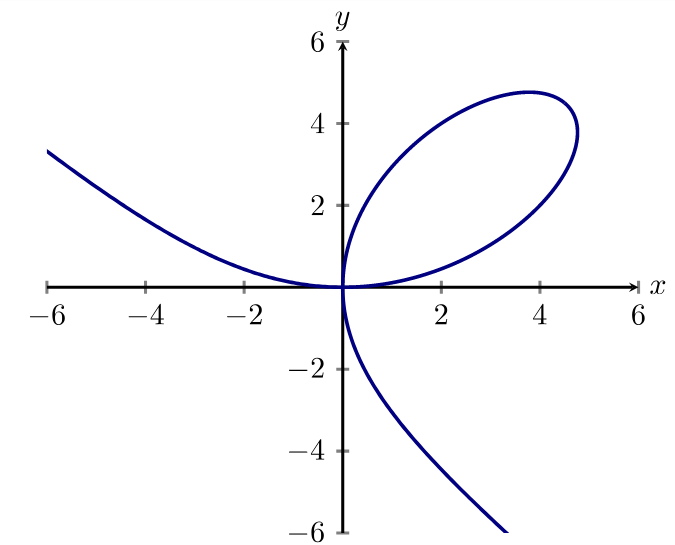
\includegraphics{3.png}
\end{image}
\begin{explanation}
Let $R$ be the radius of the sphere, and let $r$ and $h$ be the base
radius and height of the cone inside the sphere.  Our goal is to
maximize the volume of the cone: $V_c=\pi r^2h/3$.  The largest $r$
could be is $R$ and the largest $h$ could be is $2R$.

Notice that the function we want to maximize, $\pi r^2h/3$, depends on
\textit{two} variables.  Our next step is to find the relationship between $r$ and $h$ and
use it to solve for one of the variables in terms of the other, so as
to have a function of only one variable to maximize.  In this problem,
the condition is apparent in the figure below.

\begin{image}
  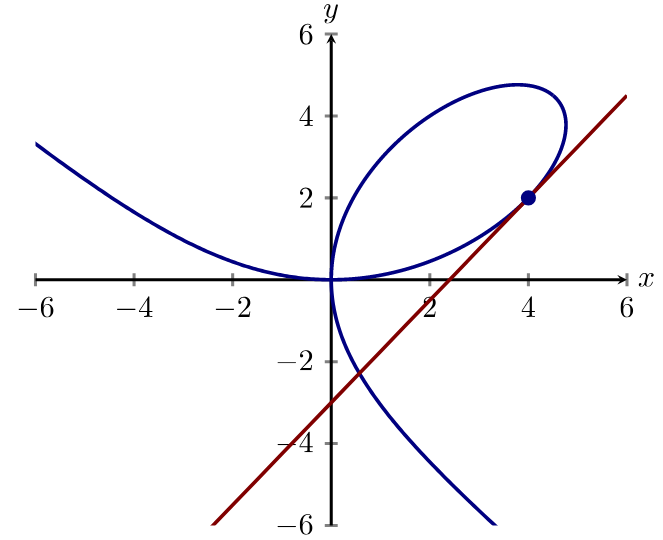
\includegraphics{4.png}
\end{image}

Apply the Pythagorean Theorem to the right triangle in the figure above to obtain

\[
r^2 + (h-R)^2=R^2.
\] 
Solve for $r^2$, since $r^2$ is found in the formula for the volume
of the cone, and find that
\[
r^2=R^2-(h-R)^2=2hR-h^2.
\]  
Substitute this into the formula for the volume of the cone to find that 
\[
 V_{\text{c}}(h)=\pi(R^2-(h-R)^2)h/3. 
 \]
By simplifying, we were able to express the volume of the cone as a function of a single variable, $h$,
\[
 V_{\text{c}}(h)=-{\pi\over3}h^3+{2\over3}\pi h^2R.
 \]

We want to maximize the function $V_{\text{c}}$ on the interval $[0,2R]$.
Since this is a continuous function on a closed interval, the maximum is attained either at a critical point or an end point.
By solving the equation 
\[
V_{\text{c}}'(h)=-\pi h^2+(4/3)\pi h R=0,
\] 
we find that the function has at $h=4R/3$ its only critical point, since $h=0$ is an end point.  We evaluate the function at all the critical and end points,
\[
V_{\text{c}}(0)=V_{\text{c}}(2R)=0,
\]

\[
V_{\text{c}}(4R/3)=(32/81)\pi R^3.
\] 

The maximum is obviously attained at $h=4R/3$ . Since the volume of the sphere is $(4/3)\pi
R^3$, the fraction of the sphere occupied by the cone is
\[
\frac{(32/81)\pi R^3}{(4/3)\pi R^3}=\frac{8}{27}\approx 30\%.
\]
\end{explanation}
\end{example}






%% From APEX
\begin{example}
  A power line needs to be run from a power station located on the
  beach to an offshore facility.
  \begin{image}
    \includegraphics{5.png}
  \end{image}
  It costs \$50/ft. to run a power line along the land, and \$130/ft. to
  run a power line under water. How much of the power line should be run
  along the land to minimize the overall cost? What is the minimal cost?
  \begin{explanation}
    There are two immediate solutions that we could consider, each of
    which we will reject through ``common sense.'' First, we could
    minimize the distance by directly connecting the two locations with a
    straight line. However, this requires that all the wire be laid
    underwater, the most costly option. Second, we could minimize the
    underwater length by running a wire all 5000 ft. along the beach,
    directly across from the offshore facility. This has the undesired
    effect of having the longest distance of all, probably ensuring a
    nonminimal cost.
    
    The optimal solution likely has the line being run along the
    ground for a while, then underwater, as the figure implies. We
    need to label our unknown distances: the distance run along the
    ground and the distance run underwater. Recognizing that the
    underwater distance can be measured as the hypotenuse of a right
    triangle, we can label our figure as follows
      \begin{image}
	\includegraphics{6.png}
      \end{image}
      By choosing $x$ as we did, we make the expression under the
      square root simple. We now create the cost function:
    \[
    \begin{array}{ccc}
      \text{Cost} = & & \\
      \text{land cost} & + & \text{water cost} \\
      \text{\$50}\times \text{land distance} &+& \text{\$130}\times \text{water distance} \\
      50(5000-x) &+& 130\sqrt{x^2+1000^2}.\\
    \end{array}
    \]
    So we have
    \[
    c(x) = 50(5000-x)+ 130\sqrt{x^2+1000^2}.
    \]
    This function only makes sense on the interval $[0,5000]$. While
    we are fairly certain the endpoints will not give a minimal cost,
    we still evaluate $c(x)$ at each to verify.
    \[
    c(0) = 380000 \quad\quad c(5000) \approx 662873.
    \]
    We now find the critical points of $c(x)$. We compute $c'(x)$ as
    \[
    c'(x) = -50+\frac{\answer[given]{130x}}{\sqrt{x^2+1000^2}}.
    \]
    Recognize that this is never undefined. Setting $c'(x)=0$ and solving
    for $x$, we have:
    \begin{align*}
      -50+\frac{130x}{\sqrt{x^2+1000^2}} &= 0 \\
      \frac{130x}{\sqrt{x^2+1000^2}}  &= 50\\
      \frac{130^2x^2}{x^2+1000^2} &= 50^2\\
      130^2x^2 &= 50^2(x^2+1000^2) \\
      130^2x^2-50^2x^2 &= 50^2\cdot1000^2\\
      (130^2-50^2)x^2 &= 50000^2\\
      x^2 &= \frac{50000^2}{130^2-50^2}\\
      x &= \frac{50000}{\sqrt{130^2-50^2}}\\
      x &= \frac{50000}{120},
    \end{align*}
    Evaluating $c(x)$ at $x=416.67$ gives a cost of about
    $\$370000$. The distance the power line is laid along land is
    $5000-416.67 = 4583.33\unit{ft}$ and the underwater distance is
    $\sqrt{416.67^2+1000^2} \approx 1083\unit{ft}$.
  \begin{onlineOnly}
  We can confirm out results by looking at the graph of $y=c(x)$: 
  \[
  \graph[xmin=0, xmax=5000, ymin=0, ymax=800000]{y=50(5000-x)+130\sqrt{x^2+1000000}}
  \]
  \end{onlineOnly}
  \end{explanation}
\end{example}




We now work a similar problem without concrete numbers.






\begin{example}\label{exam:sand and road}
  Suppose you want to reach a point $A$ that is located across the
  sand from a nearby road.
\begin{image}
  \includegraphics{7.png}
\end{image}
  Suppose that the road is straight, and $b$ is the distance from $A$
  to the closest point $C$ on the road.  Let $v$ be your speed on the
  road, and let $w$, which is less than $v$, be your speed on the
  sand.  Right now you are at the point $D$, which is a distance $a$
  from $C$.  At what point $B$ should you turn off the road and head
  across the sand in order to minimize your travel time to $A$?
  \begin{explanation}
    Let $x$ be the distance short of $C$ where you turn off, the distance
    from $B$ to $C$.  We want to minimize the total travel time.  Recall
    that when traveling at constant velocity, time is distance divided by
    velocity.

    You travel the distance from $D$ to $B$ at speed $v$, and then the
    distance from $B$ to $A$ at speed $w$.  The distance from $D$ to $B$
    is $a-x$. By the Pythagorean theorem, the distance from $B$ to $A$
    is
    \[
    \sqrt{x^2+b^2}.
    \] 
Hence the total time for the trip is
\[
T(x)=\frac{a-x}{v}+\frac{\sqrt{x^2+b^2}}{w}.
\]
We want to find the minimum value of $T$ when $x$ is between 0 and
$a$.  As usual we set $T'(x)=0$ and solve for $x$. Write
\[
  T'(x)=\answer[given]{-1/v+\frac{x}{w\sqrt{x^2+b^2}}} =0.
\]
We find that 
\[
x=\frac{wb}{\sqrt{v^2-w^2}}
\]
Notice that $a$ does not appear in the last expression, but $a$ is not
irrelevant, since we are interested only in critical values that are
in $[0,a]$, and $wb/\sqrt{v^2-w^2}$ is either in this interval or not.
If it is, we can use the second derivative to test it:
\[
T''(x) = \answer[given]{\frac{b^2}{(x^2+b^2)^{3/2}w}}.
\]
Since this is always positive there is a local minimum at the critical
point, and so it is a global minimum as well.

If the critical value is not in $[0,a]$ it is larger than $a$. In this
case the minimum must occur at one of the endpoints. We can compute
\begin{align*}
T(0)&={a\over v}+{b\over w} \\
T(a)&={\sqrt{a^2+b^2}\over w} 
\end{align*}
but it is difficult to determine which of these is smaller by direct
comparison. If, as is likely in practice, we know the values of $v$,
$w$, $a$, and $b$, then it is easy to determine this. With a little
cleverness, however, we can determine the minimum in general. We have seen that
$T''(x)$ is always positive, so the derivative $T'(x)$ is always increasing.
We know that at $wb/\sqrt{v^2-w^2}$ the derivative is zero, so for
values of $x$ less than that critical value, the derivative is
negative. This means that $T(0)>T(a)$, so the minimum occurs when $x=a$.

So the upshot is this: If you start farther away from $C$ than
$wb/\sqrt{v^2-w^2}$ then you always want to cut across the sand 
when you are a distance $wb/\sqrt{v^2-w^2}$ from point $C$. If you
start closer than this to $C$, you should cut directly across the sand.
\end{explanation}
\end{example}


%% Edited from APEX
With optimization problems you will see a variety of situations that
require you to combine problem solving skills with calculus. Focus on
the \textit{process}.  One must learn how to form equations from
situations that can be manipulated into what you need. Forget
memorizing how to do ``this kind of problem'' as opposed to ``that
kind of problem.''
\begin{quote}
  \textbf{Learning a process will benefit one far more than memorizing
    a specific technique.}
\end{quote}



\end{document}
